% P3 v3.2.0-r2 structural recovery: focused DESI DR1 candidate-catalog paper.
% Canonical source for the ApJS submission track.
% Compile: latexmk -pdf -interaction=nonstopmode -halt-on-error paper3_apjs.tex

\documentclass[twocolumn]{aastex701}
\usepackage{amsfonts}
\usepackage{amsmath}
\usepackage{bm}
\usepackage{booktabs}
\usepackage{longtable}
\usepackage{multirow}

\setcitestyle{numbers,square,comma}
\newcommand{\repoBase}{https://github.com/Hubify-Projects/bigbounce/blob/main}
\newcommand{\artifact}[1]{\href{\repoBase/#1}{\nolinkurl{#1}}}
\newcommand{\paperVersion}{v3.2.0-r2}
\newcommand{\releaseTag}{p3-v3.2.0-r2}
\newcommand{\releaseRevision}{1a9e85ee004894956665444b4f110111f1090b79}
\hypersetup{colorlinks=true,linkcolor=blue!60!black,citecolor=blue!60!black,urlcolor=blue!60!black}

\begin{document}

\title{A Public-ID-Rejoinable DESI DR1 Anomaly-Candidate Catalog:\\
181 Warning-Free Primary Spectra from a Reproducible Positional Recovery}

\author{Houston Golden}
\affiliation{Independent Researcher, Los Angeles, California, USA}
\email{houston@hubify.com}
\date{July 14, 2026 --- \paperVersion}

\begin{abstract}
Anomaly searches become reusable catalogs only when rows trace public archive objects and the
selection function is reconstructable.  We recover candidates from a historical DESI anomaly
stream whose legacy identifiers mixed public-looking values with internal hashes.  Starting
from 190,015 positional clusters containing a DESI member, we stream all 28,425,963 rows of the
public DESI Data Release 1 (DR1) pixel-based redshift catalog in 200,000-row chunks, read 18
columns, and query a spherical-coordinate $k$-d tree.  The predeclared parent selection is a
$1\arcsec$ match to a main-survey row carrying at least one LRG, ELG, QSO, BGS\_ANY, or MWS\_ANY
\texttt{DESI\_TARGET} bit.  It reproduces exactly 20,299,155 eligible DESI rows and 2,468
positional matches.  Requiring the global primary redshift row leaves 2,448; requiring
\texttt{ZWARN}=0 leaves 181 unique public \texttt{TARGETID}s.  These 181 rows form the \paperVersion{}
release.  They comprise 157 Redrock GALAXY, 23 QSO, and one STAR classifications; spectral type
was not a selection cut.  Of the released matches, 170 are within
$0.1\arcsec$ and 11 lie between $0.1\arcsec$ and $1\arcsec$; a quality-tier column exposes this
tail without silently changing the declared match.  Every released row and all 18 carried DESI
fields were re-read from their recorded FITS row and compared exactly.  The release includes the
Parquet catalog, dictionary, code, waterfall, checksums, and provenance.  This is a reproducible
follow-up list, not validated detections or an unbiased sample for anomaly-rate inference.
\end{abstract}

\keywords{catalogs --- surveys --- methods: data analysis --- methods: statistical --- galaxies: spectra --- quasars: general}

\section{Introduction}\label{sec:introduction}

Spectroscopic surveys make it possible to search for unusual objects at scales that cannot be
inspected manually.  Reconstruction models, latent-variable models, and other outlier methods
have consequently been applied to SDSS and DESI spectra \citep{Baron2017,Liang2023,Nicolaou2026}.
Their scientific value, however, depends on a distinction that is easy to blur: an unusual model
score is a candidate-selection signal, whereas an archive-resolvable object with auditable
quality metadata is a usable catalog row.  Neither is, by itself, a validated astrophysical
detection.

This paper addresses that distinction through a structural recovery.  An earlier multi-survey
anomaly product contained DESI sky positions, anomaly scores, and residual summaries, but most
legacy identifiers were internal hashes rather than public DESI \texttt{TARGETID}s.  A catalog
whose coordinates cannot be joined deterministically to public spectra is difficult to verify,
extend, or cite object by object.  The earlier product also mixed survey-specific selection
functions.  Treating its aggregate row count as a homogeneous scientific sample would therefore
be misleading even if every row were numerically correct.

We replace that scope with one falsifiable deliverable: a DESI DR1 science-target candidate
catalog whose public identifiers and carried metadata can be rejoined exactly.  The recovery
uses the historical anomaly stream only as a source of coordinates and score metadata.  Public
identity, targeting information, primary-row status, redshift metadata, and fit warnings all
come from the current public DESI DR1 redshift catalog \citep{DESI2025DR1}.  The result is a small
quality-controlled follow-up set rather than a claim about the prevalence, novelty, or physical
origin of anomalous spectra.

The contributions are:
\begin{enumerate}
\item a memory-bounded, checkpointed join of 190,015 DESI-containing anomaly clusters to the
28.4 million-row DR1 redshift catalog;
\item an exact reproduction of the previously quoted 2,468-row main-survey science-bit cohort;
\item a declared quality waterfall yielding 181 warning-free global-primary candidates;
\item a public-ID release with exact field-by-field source-row validation; and
\item a clean \paperVersion{} bundle containing only this DESI product and the artifacts required to audit it.
\end{enumerate}

Section~\ref{sec:data} defines the two inputs.  Section~\ref{sec:method} specifies the join,
selection, and duplicate rules.  Section~\ref{sec:results} describes the released cohort without
interpreting it as a population measurement.  Sections~\ref{sec:selection} and
\ref{sec:reproducibility} make the selection biases and reproducibility checks explicit.

\section{Inputs and Scope}\label{sec:data}

\subsection{Historical anomaly-cluster substrate}\label{sec:anomaly-input}

The starting cluster table contains 378,480 coordinate clusters produced by a prior positional
deduplication.  Exactly 190,015 have a survey-membership string containing \texttt{desi\_dr1};
190,005 are DESI-only clusters, eight also contain an SDSS member, and two also contain a LAMOST
member.  Those historical cross-survey labels are retained only as provenance columns.  They do
not enter the \paperVersion{} selection and no non-DESI table is included in the new release.

The accompanying DESI anomaly table has 195,829 rows with an internal identifier, right
ascension, declination, a scalar score $S$, the band producing the largest residual, and three
residual summaries.  The legacy identifier is not treated as a public key.  It mixes positive
public-looking values with internal hashed values; 169,611 of the 195,829 values are negative.
Within the released 181-row cohort, ten legacy identifiers are negative.  This behavior is
preserved as audit history in \texttt{original\_internal\_tid}, while the recovered public
\texttt{targetid} is the only archive join key recommended for users.

When a cluster contains more than one DESI anomaly member, its canonical historical member is
the one with the largest original score; ties are resolved by the smaller original row number.
The score and residual fields are carried forward verbatim as ranking metadata.  They are not
recomputed in this work, and they are not interpreted as calibrated probabilities, physical
significances, or novelty measures.

Exactly one released cluster has more than one historical anomaly member:
\texttt{P3-DESI-000030} (\texttt{cluster\_id}=71390, \texttt{n\_detections}=2).  Its recovered
public target is $0.979656\arcsec$ from the cluster coordinate but $1.979009\arcsec$ from the
canonical original DESI member.  The public $1\arcsec$ selection is explicitly the target-to-cluster
separation, not a target-to-original-member cut.  The release stores both quantities as
\texttt{match\_separation\_arcsec} and \texttt{original\_member\_separation\_arcsec}.

\subsection{Public DESI DR1 redshift catalog}\label{sec:desi-input}

The public identity substrate is the \texttt{ZCATALOG} binary-table HDU (extension 1) of
\texttt{zall-pix-iron.fits} from DESI DR1.  The local file has
28,425,963 rows and 22,371,272,640 bytes.  Its SHA-256 is
\texttt{2d95ad99361039b556c402b49e0e7c84\allowbreak df5f00106dc5731d44476a58b128b49b}, equal to the
value in DESI's current official checksum list.  The FITS table contains repeat observations,
survey and program labels, targeting bitmasks, Redrock redshift products, and flags defining
primary rows.  We read only the fields listed in Table~\ref{tab:desi-fields}; no 21~GB in-memory
table is formed.

\begin{deluxetable*}{lll}
\tablecaption{DESI fields read from each streamed FITS chunk\label{tab:desi-fields}}
\tablehead{Group & Fields & Role in this work}
\startdata
Identity/position & \texttt{TARGETID}, \texttt{TARGET\_RA}, \texttt{TARGET\_DEC} & public rejoin and angular match \\
Observing context & \texttt{SURVEY}, \texttt{PROGRAM} & main-survey selection and description \\
Targeting & \texttt{DESI\_TARGET}, \texttt{BGS\_TARGET}, \texttt{MWS\_TARGET}, \texttt{SCND\_TARGET} & science-bit selection and raw metadata \\
Redshift fit & \texttt{Z}, \texttt{ZWARN}, \texttt{SPECTYPE}, \texttt{DELTACHI2} & quality gate and descriptive metadata \\
Coadd status & \texttt{COADD\_FIBERSTATUS} & descriptive quality cross-check \\
Primary flags & \texttt{MAIN\_NSPEC}, \texttt{MAIN\_PRIMARY}, \texttt{ZCAT\_NSPEC}, \texttt{ZCAT\_PRIMARY} & repeat accounting and final primary gate \\
\enddata
\tablecomments{Column names follow the public DESI zcatalog.  Only \texttt{SURVEY},
\texttt{DESI\_TARGET}, \texttt{ZCAT\_PRIMARY}, and \texttt{ZWARN} enter the final Boolean selection;
coordinates enter the positional join.  \texttt{SPECTYPE} and \texttt{Z} are not selection cuts.}
\end{deluxetable*}

\section{Recovery and Selection Method}\label{sec:method}

\subsection{Memory-bounded positional join}\label{sec:join}

All cluster coordinates are converted from $(\alpha,\delta)$ to three-dimensional unit vectors,
\begin{equation}
\boldsymbol{x}=(\cos\delta\cos\alpha,\cos\delta\sin\alpha,\sin\delta),
\end{equation}
and indexed once with a \texttt{cKDTree}.  The FITS table is then traversed in blocks of 200,000
rows using \texttt{fitsio}.  Numeric arrays are converted from FITS big-endian storage to native
byte order before Parquet serialization.  Within each block we first apply the survey and target
bit mask, convert the remaining coordinates to unit vectors, and query the nearest cluster.
Chord distances are converted back to great-circle arcseconds.  Only matches within the
predeclared $1\arcsec$ radius are retained.

Each completed block is written atomically to a small Parquet part.  A JSON checkpoint records
the input signature, completed block starts, cumulative row counts, and the last completed row;
a fsynced JSON-lines progress file records the same counts with timestamps.  Restarting with the
same signature skips completed parts.  A changed FITS path, size, column set, radius, chunk size,
or cluster count invalidates the checkpoint rather than silently mixing runs.  The full scan took
97.1~s on the audit machine and retained only 2,468 match rows.  Runtime is reported for
reproducibility, not as a cross-platform benchmark.

\subsection{Science-target parent cohort}\label{sec:parent-selection}

The parent cohort uses the exact historical bitmask definition so that the earlier 2,468 count
can be tested.  A row is eligible when
\begin{equation}
\begin{split}
&\texttt{SURVEY}=\texttt{main},\\
&\texttt{DESI\_TARGET}\mathbin{\&}
\left(2^0\,|\,2^1\,|\,2^2\,|\,2^{60}\,|\,2^{61}\right)\ne0,
\end{split}
\end{equation}
where bits 0, 1, 2, 60, and 61 denote LRG, ELG, QSO, BGS\_ANY, and MWS\_ANY, respectively.
These classes are not mutually exclusive.  The streamed scan finds 20,299,155 eligible rows,
exactly reproducing the historical denominator.  Their nearest-neighbor join yields 2,468 rows
within $1\arcsec$, exactly reproducing the historical match count.  This agreement tests the
coordinate transform, endian-correct bitmask evaluation, row traversal, and radius together.

\subsection{Quality cohort and duplicate rules}\label{sec:quality-selection}

The public redshift catalog may contain multiple rows associated with one target.  We therefore
require \texttt{ZCAT\_PRIMARY}=true, the global primary redshift-row flag.  We then require
\texttt{ZWARN}=0.  This latter gate is intentionally conservative: it removes any Redrock fit
carrying a warning bit.  We do not require a particular \texttt{SPECTYPE}, redshift range, or
minimum \texttt{DELTACHI2}; imposing such post-hoc cuts would redefine which anomaly morphologies
survive.

Before the final gates, a FITS row is assigned to its nearest anomaly cluster only.  Within any
cohort, duplicate cluster matches are ordered by smaller angular separation, larger
\texttt{DELTACHI2}, smaller \texttt{TARGETID}, and smaller FITS row.  A second pass uses the same
ordering to enforce one row per public \texttt{TARGETID}.  No tie-breaking is needed in the final
cohort, but publishing the rule makes reruns deterministic.  The final 181 rows have unique
candidate IDs, cluster IDs, public \texttt{TARGETID}s, and FITS row numbers.

\subsection{Match-quality tier}\label{sec:match-tier}

The $1\arcsec$ radius was fixed before inspecting the quality cohort and is retained for exact
historical count reproduction.  Most recovered coordinates agree much more closely: 170 of 181
are separated by at most $0.1\arcsec$.  Eleven lie between $0.1\arcsec$ and $1\arcsec$, including
eight above $0.5\arcsec$ and five above $0.75\arcsec$; the maximum is $0.9906\arcsec$.  Rather than
silently deleting these valid-by-definition matches, we publish \texttt{match\_quality\_tier} with
values \texttt{coordinate\_consistent\_le\_0p1arcsec} and
\texttt{positional\_match\_gt\_0p1\_le\_1arcsec}.  Users can reproduce either the declared catalog
or the 170-row high-coordinate-consistency subset.

\section{Catalog Results}\label{sec:results}

\subsection{Selection waterfall}\label{sec:waterfall}

Table~\ref{tab:waterfall} and Figure~\ref{fig:waterfall} give the full waterfall.  Of the 2,468
parent matches, only 20 are removed by the global-primary requirement.  The dominant reduction
is \texttt{ZWARN}=0: 2,267 of the 2,448 primary rows carry at least one warning bit, leaving 181.
Requiring \texttt{MAIN\_PRIMARY} in addition changes nothing; requiring
\texttt{COADD\_FIBERSTATUS}=0 after the adopted gates also changes nothing.  These equalities are
reported as cross-checks, not as independent evidence that the sample is unbiased.

\begin{deluxetable}{lr}
\tablecaption{Declared selection waterfall\label{tab:waterfall}}
\tablehead{Stage & Rows}
\startdata
DESI-containing anomaly clusters & 190,015 \\
Main science-bit DESI rows searched & 20,299,155 \\
$\leq1\arcsec$ positional matches & 2,468 \\
Remove non-\texttt{ZCAT\_PRIMARY} & $-20$ \\
Global-primary matches & 2,448 \\
Remove primary rows with \texttt{ZWARN}$\ne0$ & $-2,267$ \\
Released candidates & \textbf{181} \\
\enddata
\tablecomments{The 181-row release is 7.33\% of the positional science-bit cohort.}
\end{deluxetable}

\begin{figure*}
\centering
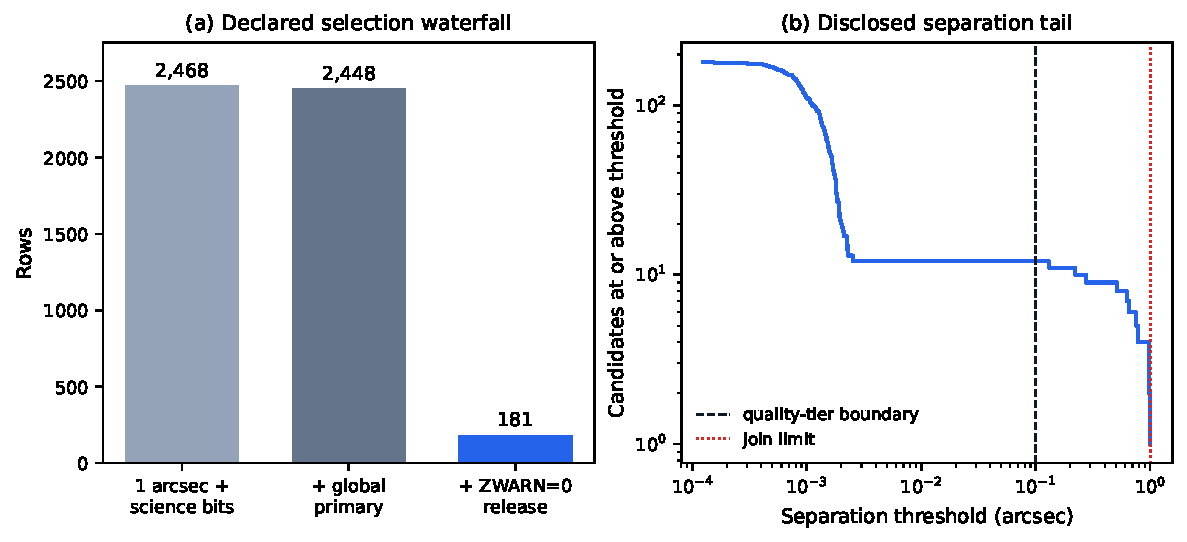
\includegraphics[width=0.82\textwidth]{figures/p3_v320_selection_waterfall.pdf}
\caption{\textit{Left:} Selection waterfall from the exact historical bitmask cohort to the
warning-free global-primary release.  \textit{Right:} Number of released candidates at or above
each positional separation.  The dashed line marks the published quality-tier boundary; the
dotted line is the predeclared join limit.\label{fig:waterfall}}
\end{figure*}

The large \texttt{ZWARN} reduction is scientifically important.  An anomaly-selected spectrum is
more likely than an ordinary spectrum to be difficult for a standard template-fitting pipeline.
Consequently, the warning-free subset is cleaner for catalog-level redshift metadata but is not
a random subset of all unusual spectra.  This tradeoff motivates the restricted interpretation
in Section~\ref{sec:selection}.

\subsection{Descriptive composition}\label{sec:composition}

Redrock classifies 157 released rows as GALAXY, 23 as QSO, and one as STAR.  The observing programs
are 162 dark and 19 bright.  Target-bit labels are overlapping: 157 rows carry ELG, 18 BGS\_ANY,
seven QSO, one LRG, and one MWS\_ANY; a row can contribute to more than one count.  These values
describe the catalog after selection.  They do not measure selection efficiencies by class
because the relevant class-specific parent denominators and warning mechanisms have not been
modeled.

The redshift metadata span $-0.00034\le z\le6.0878$, with quartiles 0.616, 1.108, and 1.401.
Two rows have $z<0$; 36 lie in $0\le z<0.5$, 36 in $0.5\le z<1$, 76 in $1\le z<1.5$, eight in
$1.5\le z<2$, 13 in $2\le z<3$, and ten at $z\ge3$.  The two small negative values are retained
because \texttt{ZWARN}=0 is the declared quality criterion and no physical-redshift cut was
predeclared.  Users interested in a positive-redshift science subset should add that cut
explicitly and report the resulting 179 rows.

The original anomaly-score range in the release is 5.0006--7.7057, with a median of 5.3244.  This
narrow range is inherited from the historical anomaly threshold.  We do not convert it to a
Gaussian significance or compare it across models.  Figure~\ref{fig:overview} shows the sky,
redshift, score, and separation metadata without attaching a detection interpretation.

\begin{figure*}
\centering
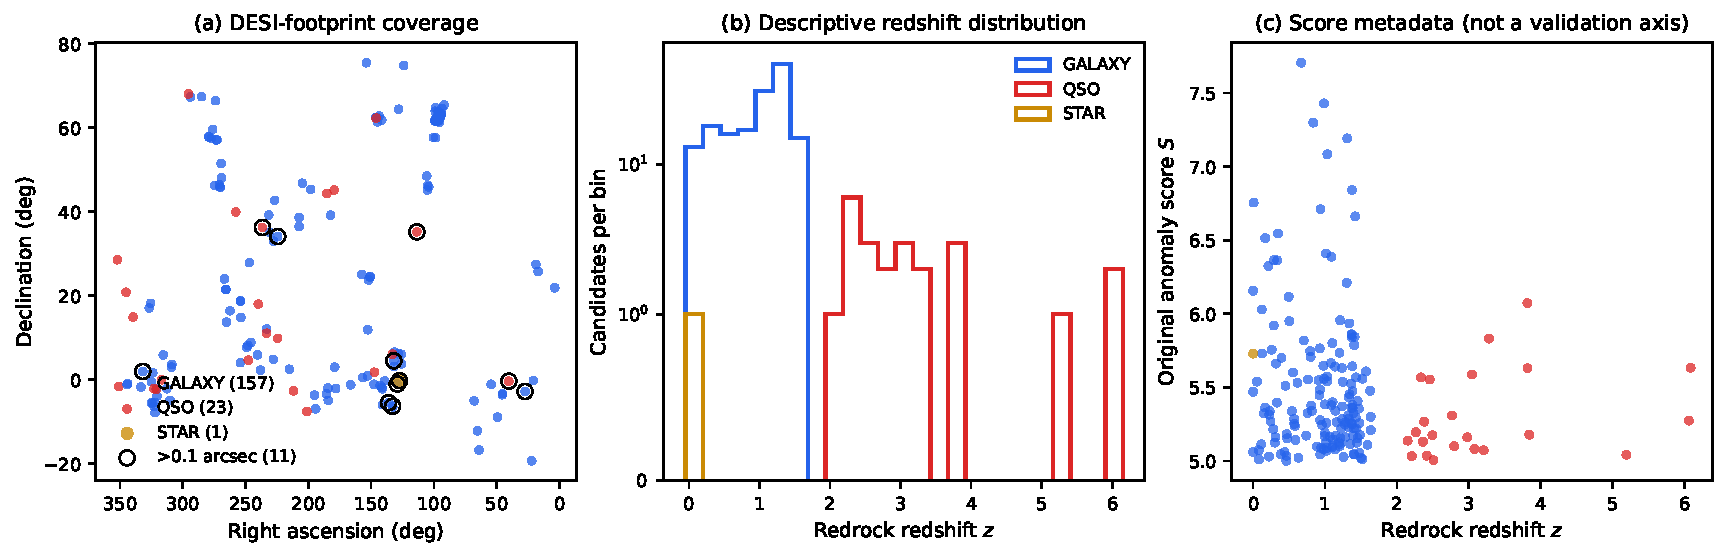
\includegraphics[width=\textwidth]{figures/p3_v320_catalog_overview.pdf}
\caption{Released \paperVersion{} candidates.  (a) DESI-footprint sky distribution colored by descriptive
Redrock \texttt{SPECTYPE}; open circles mark the 11 rows in the $0.1$--$1\arcsec$ separation tier.
(b) Redshift metadata by spectral type.  (c) Historical anomaly score versus Redrock redshift.
Neither \texttt{SPECTYPE} nor redshift was used to select the release, and the score is not a
calibrated physical significance.\label{fig:overview}}
\end{figure*}

\subsection{Sky and positional coverage}\label{sec:sky}

The released positions range from $3.73^\circ$ to $352.15^\circ$ in right ascension and
$-19.31^\circ$ to $75.49^\circ$ in declination.  There are 134 candidates north and 47 south of
the celestial equator.  All twelve 30-degree right-ascension bins are occupied, while four of
six coarse equal-area declination bins are occupied.  These summaries demonstrate geographic
coverage within the input, not isotropy.  The footprint is inherited from DESI DR1 and the
historical anomaly sample; no all-sky uniformity correction is attempted.

The median positional separation is $0.00127\arcsec$, with quartiles $0.00083\arcsec$ and
$0.00167\arcsec$.  The abrupt tail of 11 larger separations is why both the continuous separation
and categorical quality tier are released.  Positional coincidence inside $1\arcsec$ supports a
catalog association, but it does not prove that the historical anomaly-row identity and public
spectrum are physically identical in crowded or blended fields.  Those 11 rows are natural
priorities for image-level and spectrum-level manual verification.

\subsection{Example rows}\label{sec:examples}

Table~\ref{tab:examples} lists the twelve highest historical scores only to illustrate the schema.
Rank in this table is not a recommendation that the objects are novel or astrophysically
important.  The complete machine-readable catalog contains all 181 rows.

\begin{deluxetable*}{lrrrrrrr}
\tablecaption{Highest-score example rows from the released catalog\label{tab:examples}}
\tablehead{Candidate & TARGETID & R.A. & Decl. & Type & $z$ & $S$ & Sep. (arcsec)}
\startdata
P3-DESI-000001 & 39633349869831142 & 272.82236 & 57.12256 & GALAXY & 0.668 & 7.71 & 0.001 \\
P3-DESI-000002 & 39627706974869534 & 45.28046 & -3.31238 & GALAXY & 0.986 & 7.43 & 0.002 \\
P3-DESI-000003 & 39627895609492977 & 131.94836 & 4.51377 & GALAXY & 0.838 & 7.30 & 0.274 \\
P3-DESI-000004 & 39633407088529181 & 97.49930 & 61.65664 & GALAXY & 1.310 & 7.19 & 0.001 \\
P3-DESI-000005 & 39627636166626827 & 132.90847 & -6.30883 & GALAXY & 1.033 & 7.08 & 0.991 \\
P3-DESI-000006 & 39633418404759790 & 95.13019 & 62.74366 & GALAXY & 1.376 & 6.84 & 0.000 \\
P3-DESI-000007 & 39636182677589446 & 64.05184 & -16.74091 & GALAXY & 0.006 & 6.76 & 0.002 \\
P3-DESI-000008 & 39633407096917948 & 98.59444 & 61.74095 & GALAXY & 0.938 & 6.71 & 0.000 \\
P3-DESI-000009 & 39627748041295714 & 333.31949 & -1.73961 & GALAXY & 1.420 & 6.66 & 0.001 \\
P3-DESI-000010 & 39633186518469218 & 104.94924 & 46.24594 & GALAXY & 0.347 & 6.55 & 0.001 \\
P3-DESI-000011 & 39633063570837088 & 231.50666 & 39.22886 & GALAXY & 0.167 & 6.51 & 0.001 \\
P3-DESI-000012 & 39627877414602764 & 125.74951 & 3.78702 & GALAXY & 1.015 & 6.41 & 0.002 \\
\enddata
\tablecomments{R.A. and declination are ICRS degrees.  Type and $z$ are public Redrock metadata.
$S$ is preserved historical anomaly-score metadata.  Values are rounded for display only.}
\end{deluxetable*}

\section{Selection Function and Appropriate Use}\label{sec:selection}

\subsection{What the catalog selects}\label{sec:what-selects}

The release is the intersection of four operations: membership in a historical anomaly-cluster
substrate, positional coincidence with a public DESI row inside $1\arcsec$, membership in the
declared main-survey science-bit parent, and the \texttt{ZCAT\_PRIMARY}/\texttt{ZWARN}=0 quality
gates.  It is therefore conditional on the historical anomaly model, preprocessing, score
threshold, survey footprint, target selection, public zcatalog construction, and Redrock warning
behavior.  The present work makes those operations reproducible; it does not make them ignorable.

In particular, the released fraction $181/2468=7.33\%$ must not be called an anomaly rate, a
validation efficiency, or a purity estimate.  The numerator is conditioned on warning-free
template fits, while the denominator contains the very spectra for which template fitting may be
difficult.  A population analysis would require at least the class-, magnitude-, redshift-,
signal-to-noise-, and warning-dependent inclusion probabilities for both the historical anomaly
stage and the DESI rejoin stage.  Those quantities are not available in this release.

\subsection{Recommended uses}\label{sec:uses}

The catalog is designed for:
\begin{itemize}
\item deterministic retrieval of 181 public DESI spectra by \texttt{TARGETID};
\item manual or automated spectral vetting using the full public data products;
\item testing alternative anomaly models on a fixed, warning-free candidate list;
\item follow-up prioritization using continuous score, separation, target-bit, and redshift metadata; and
\item reproducibility exercises in archive recovery and catalog selection.
\end{itemize}

It is not designed for estimating an anomaly occurrence rate, claiming new object classes,
measuring cosmological parameters, or comparing raw counts with a differently selected survey.
No SIMBAD-based novelty fraction, process-volume multiplier, cross-survey total, or cosmological
inference is part of \paperVersion{}.  Establishing novelty requires object-by-object literature and archive
review beyond a coordinate database match.  Establishing a physical anomaly requires inspection
of calibrated spectra, masks, observing conditions, and repeat observations.

\subsection{Relationship to prior DESI anomaly searches}\label{sec:prior}

Prior DESI studies have demonstrated useful outlier-search strategies for particular target
classes and data subsets \citep{Liang2023,Nicolaou2026}.  Direct candidate-count comparisons are
not meaningful here because the parent populations, preprocessing, models, thresholds, and
quality gates differ.  The contribution of \paperVersion{} is orthogonal: it converts a historically
unrejoinable coordinate-and-score product into a small public-key catalog with a fully enumerated
waterfall.  Future model comparisons can use these 181 public spectra as a common follow-up set,
but evaluation against a representative control sample would still be required.

\section{Reproducibility and Integrity Audit}\label{sec:reproducibility}

\subsection{Exact source-row rejoin}\label{sec:exact-rejoin}

The independent validator reads the released \texttt{fits\_row} values from the final Parquet,
reopens the public FITS file, and retrieves all 18 source fields listed in
Table~\ref{tab:desi-fields}.  Integer, Boolean, and string fields are compared exactly; floating
fields are also compared at zero tolerance because the Parquet values were copied directly.
All 181 rows pass all 18 field comparisons.  Independently of the released table, the validator
reconstructs the strict cohort from the 143 scan checkpoints and compares the complete
\texttt{(cluster\_id, targetid, fits\_row)} sets.  The sets are exactly equal (181 expected,
181 released, zero missing, and zero unexpected), rather than merely having equal counts.
The validator separately confirms unique candidate,
cluster, \texttt{TARGETID}, and FITS-row keys; zero null cells; main-survey membership; at least one
declared science bit; \texttt{ZCAT\_PRIMARY}=true; \texttt{ZWARN}=0; and separation at or below
$1\arcsec$.

\subsection{Provenance and checksum reconciliation}\label{sec:checksums}

The full local 22.37~GB FITS SHA-256 was recomputed.  A no-cache retrieval of DESI's current
official checksum file reports the same value.  The live FITS endpoint reports the same byte size,
an ETag of \texttt{6a516695-5356e87c0}, and a last-modified time of 2026-07-10 21:39:33 GMT.  The
machine validator issued eight live 1~MiB HTTP Range requests, including the first and last
ranges, and required for each response status 206, the exact \texttt{Content-Range}, the exact
byte count, and a SHA-256 equal to the corresponding local bytes.  All eight passed.  An older
local provenance sidecar written in May 2026 records a
different pre-replacement SHA-256.  We preserve that stale value in \texttt{PROVENANCE.json} and
explicitly exclude it from current validation rather than overwriting the history.

The two historical input Parquets are also hashed: the cluster table is
\texttt{b14deb02...d6138c643} (12,087,824 bytes) and the anomaly table is
\texttt{0a36b8d6...f103ec65} (10,514,503 bytes).  Full hashes, not abbreviated display forms, are in
the release manifest and provenance file.

\subsection{Release contents}\label{sec:release}

The clean \paperVersion{} directory contains one science table and its audit artifacts:
\begin{enumerate}
\item \nolinkurl{desi_dr1_science_anomaly_candidates_v3.2.0-r2.parquet};
\item \texttt{DATA\_DICTIONARY.md} and \texttt{README.md};
\item \texttt{COHORT\_COUNTS.json}, \texttt{QC\_REPORT.json}, and
\texttt{SELECTION\_AUDIT.json/.md};
\item exact build and independent-validation scripts;
\item \texttt{PROVENANCE.json}; and
\item \texttt{RELEASE\_MANIFEST.json} with SHA-256 and byte size for every payload file.
\end{enumerate}
The manifest hashes ten payload files and excludes itself to avoid a self-referential hash;
the directory therefore contains eleven files total.  An independent post-generation
pass recomputes every listed hash and byte count.  The release contains no Gaia, eROSITA, LAMOST,
SDSS, Planck, ACT, or heterogeneous aggregate table.  Earlier releases remain historical and are
not moved or rewritten.

\section{Limitations}\label{sec:limitations}

The catalog has six central limitations.

\textit{First, historical score lineage.}  The original score and residual columns are preserved
from the anomaly stream rather than recomputed from public spectra.  Public identifiers now make
future rescoring possible, but \paperVersion{} does not claim exact reproduction of the historical neural
network output.

\textit{Second, quality-conditioned incompleteness.}  Requiring \texttt{ZWARN}=0 removes 92.6\%
of primary positional matches.  The released list is cleaner for metadata use but incomplete by
construction and likely biased against the most difficult-to-fit spectra.

\textit{Third, positional association.}  A $1\arcsec$ match is not a proof of identity in every
field.  The 11 rows above $0.1\arcsec$ are flagged, and all users retain the continuous separation.

\textit{Fourth, no astrophysical vetting.}  Redrock class, redshift, and \texttt{DELTACHI2} are
catalog metadata.  We have not inspected every spectrum, image, mask, or repeat observation, and
we make no novelty or physical-anomaly claim.

\textit{Fifth, inherited footprint and targeting.}  The sample follows DESI DR1 coverage and the
declared target bits.  Target classes overlap, and no completeness correction is provided.

\textit{Sixth, version specificity.}  Public redshift products can be regenerated or superseded.
The release pins file size and checksum so later catalog versions can be compared rather than
silently substituted.

These limitations are not peripheral caveats: they define the valid use of the product.  The
release should be cited as a candidate catalog and reproducibility artifact.

\section{Conclusions}\label{sec:conclusions}

We have replaced a heterogeneous, public-ID-limited anomaly product with a focused DESI DR1
catalog whose selection and provenance are testable from end to end.  A memory-bounded scan of
28,425,963 public zcatalog rows exactly reproduces the prior 20,299,155-row science-bit denominator
and 2,468 one-arcsecond positional matches.  The declared global-primary and warning-free gates
yield 181 unique public \texttt{TARGETID}s.  All carried DESI fields rejoin exactly, all released
keys are unique, and every payload hash and byte size passes an independent manifest audit.

The smaller, auditable count is the catalog-integrity improvement.  It replaces an unsupported implication of
hundreds of thousands of validated detections with 181 traceable candidates and a clear account
of the 2,287 exclusions.  The release retains the full $1\arcsec$ cohort definition while exposing
the 11-row separation tail, preserves historical score metadata without turning it into a
significance, and states that the warning-free cohort is unsuitable for occurrence-rate
inference.  Its immediate purpose is reproducible spectral retrieval and follow-up.  Physical
classification is future work.

\section*{Data Availability}

The \paperVersion{} release bundle is published under the correction tag \releaseTag{} in the
public Hugging Face dataset
\url{https://huggingface.co/datasets/bamfai/bigbounce-anomaly-catalog}, path
\texttt{releases/p3-v3.2.0-r2/}.  At publication the tag resolves to commit
\texttt{\releaseRevision}; that commit hash is the authoritative immutable identifier, and exact
consumers should pin it rather than depend on a tag name alone.  All 11 remote files were
downloaded from the tagged commit and verified byte-for-byte against the local release.  The
historical \texttt{p3-v3.2.0} and \texttt{p3-v3.2.0-r1} tags and their artifacts are preserved;
\releaseTag{} is an additive successor correction.

The historical cluster and anomaly inputs are respectively
\url{https://huggingface.co/datasets/bamfai/bigbounce-anomaly-catalog/resolve/p3-v3.1.161/pathc_unique_objects.parquet}
and
\url{https://huggingface.co/datasets/bamfai/bigbounce-anomaly-catalog/resolve/p3-v3.1.161/desi_dr1_anomalies.parquet}.
Both are pinned by \texttt{p3-v3.1.161}, which resolves to commit
\texttt{cdaaa03a72c69d86f011be128d93f261dc5b39a8}; their SHA-256 values are recorded in
\texttt{PROVENANCE.json}.  The public DESI input and official checksum list are available at
\url{https://data.desi.lbl.gov/public/dr1/spectro/redux/iron/zcatalog/v1/}.  After downloading the
three named inputs, the concrete build command is:
\begin{widetext}
\begin{verbatim}
FITS_SHA256=2d95ad99361039b556c402b49e0e7c84df5f00106dc5731d44476a58b128b49b
python3 build_desi_science_catalog_v320_r2.py \
  --clusters pathc_unique_objects.parquet \
  --anomalies desi_dr1_anomalies.parquet \
  --fits zall-pix-iron.fits \
  --output-dir desi_science_catalog_v3.2.0-r2 \
  --chunk-rows 200000 \
  --fits-sha256 "$FITS_SHA256"
python3 validate_desi_science_catalog_v320_r2.py \
  --release-dir desi_science_catalog_v3.2.0-r2 \
  --fits zall-pix-iron.fits \
  --clusters pathc_unique_objects.parquet
\end{verbatim}
\end{widetext}
The expected FITS digest is assigned on one shell line and passed through an environment
variable, avoiding any copy-paste ambiguity.  The release README gives the same download, build,
and validation commands.  The source tree contains the same
scripts at \artifact{pipelines/p3\_anomaly\_engine/scripts/}.  No secret credentials or private
data are required to validate the released catalog against the public DESI file.

\section*{Software}

The build used Python 3.9.6, NumPy 1.26.4, pandas 2.1.4, SciPy 1.13.1
\citep{Virtanen2020}, fitsio 1.3.0, and PyArrow 21.0.0.  FITS is described by
the FITS standard \citep{Pence2010}.  Exact versions and the chunk size are recorded in
\texttt{PROVENANCE.json}.

\begin{acknowledgments}
This research used data obtained with the Dark Energy Spectroscopic Instrument (DESI).  DESI
construction and operations is managed by the Lawrence Berkeley National Laboratory.  This
material is based upon work supported by the U.S. Department of Energy, Office of Science,
Office of High-Energy Physics, under Contract No. DE--AC02--05CH11231, and by the National Energy
Research Scientific Computing Center, a DOE Office of Science User Facility under the same
contract.  Additional support for DESI was provided by the U.S. National Science Foundation
(NSF), Division of Astronomical Sciences under Contract No. AST-0950945 to the NSF's National
Optical-Infrared Astronomy Research Laboratory; the Science and Technology Facilities Council
of the United Kingdom; the Gordon and Betty Moore Foundation; the Heising-Simons Foundation;
the French Alternative Energies and Atomic Energy Commission (CEA); the National Council of
Humanities, Science and Technology of Mexico (CONAHCYT); the Ministry of Science and Innovation
of Spain (MICINN), and by the DESI Member Institutions:
\url{https://www.desi.lbl.gov/collaborating-institutions}.  The DESI collaboration is honored to
be permitted to conduct scientific research on I'oligam Du'ag (Kitt Peak), a mountain with
particular significance to the Tohono O'odham Nation.  Any opinions, findings, and conclusions
or recommendations expressed in this material are those of the author and do not necessarily
reflect the views of the U.S. National Science Foundation, the U.S. Department of Energy, or
any of the listed funding agencies.

The analysis benefited from automated code and manuscript review; all catalog assertions
reported here were checked against machine-readable artifacts, and no review-system output was
accepted as evidence without a local or public-source verification.
\end{acknowledgments}

\begin{thebibliography}{20}

\bibitem{DESI2025DR1}
DESI Collaboration, ``Data Release 1 of the Dark Energy Spectroscopic Instrument,''
Astron.\ J.\ \textbf{171}, 285 (2026),
\href{https://doi.org/10.3847/1538-3881/ae4c43}{doi:10.3847/1538-3881/ae4c43},
arXiv:2503.14745.

\bibitem{Baron2017}
D.\ Baron and D.\ Poznanski, ``The weirdest SDSS galaxies: results from an outlier detection
algorithm,'' Mon.\ Not.\ R.\ Astron.\ Soc.\ \textbf{465}, 4530 (2017).

\bibitem{Liang2023}
Y.\ Liang et al., ``Outlier Detection in the DESI Bright Galaxy Survey,''
Astrophys.\ J.\ Lett.\ \textbf{956}, L6 (2023), arXiv:2307.07664.

\bibitem{Nicolaou2026}
C.\ Nicolaou et al., ``Identifying Anomalous DESI Galaxy Spectra with a Variational Autoencoder,''
Mon.\ Not.\ R.\ Astron.\ Soc.\ \textbf{547}(2), stag010 (2026),
\href{https://doi.org/10.1093/mnras/stag010}{doi:10.1093/mnras/stag010},
arXiv:2506.17376.

\bibitem{Virtanen2020}
P.\ Virtanen et al., ``SciPy 1.0: Fundamental Algorithms for Scientific Computing in Python,''
Nat.\ Methods \textbf{17}, 261 (2020).

\bibitem{Pence2010}
W.\ D.\ Pence, L.\ Chiappetti, C.\ G.\ Page, R.\ A.\ Shaw, and E.\ Stobie,
``Definition of the Flexible Image Transport System (FITS), version 3.0,''
Astron.\ Astrophys.\ \textbf{524}, A42 (2010).

\end{thebibliography}

\clearpage
\appendix

\section{Executable Selection Specification}\label{app:selection}

For clarity, the released cohort can be represented by the following ordered specification:
\begin{enumerate}
\item Select the 190,015 historical clusters with \texttt{desi\_dr1} in their survey membership.
\item For each cluster, select the highest-score DESI historical member, breaking ties by source row.
\item Stream public zcatalog rows and retain
\texttt{SURVEY==main} with at least one declared \texttt{DESI\_TARGET} bit.
\item Assign each eligible zcatalog row to its nearest cluster in spherical unit-vector space.
\item Retain separations $\le1\arcsec$.
\item Within a cohort, keep the nearest row per cluster; break ties by descending
\texttt{DELTACHI2}, ascending \texttt{TARGETID}, and ascending FITS row.
\item Apply the same ordering to keep one cluster per \texttt{TARGETID}.
\item Require \texttt{ZCAT\_PRIMARY}=true and \texttt{ZWARN}=0.
\item Label separation $\le0.1\arcsec$ as coordinate-consistent and the remaining declared
$1\arcsec$ matches as the positional tail.
\item Sort by \texttt{cluster\_id} and assign sequential release-local candidate IDs.
\end{enumerate}

The script writes checkpoint parts before forming the final cohort.  Thus the selection counts
can be inspected independently of the manuscript and an interrupted full-catalog scan can resume
without replaying completed chunks.

\section{Column Groups}\label{app:columns}

The release contains 43 columns after addition of the separation-quality tier and the explicit
target-to-original-member separation.  The authoritative
field-by-field descriptions and storage dtypes are in \texttt{DATA\_DICTIONARY.md}.  The two
tables below define the public and historical field groups without duplicating them in a third
summary table.

\clearpage
\refstepcounter{table}\label{tab:public-fields}
\begin{center}
\textbf{Table \thetable.} Release and public-DESI field definitions

\smallskip
\scriptsize
\begin{tabular}{p{0.25\textwidth}p{0.68\textwidth}}
\toprule
Column & Definition \\
\midrule
\texttt{candidate\_id} & Stable release-local ID ordered by cluster ID. \\
\texttt{fits\_row} & Zero-based row in the public DR1 ZCATALOG extension used by the exact rejoin audit. \\
\texttt{cluster\_table\_row} & Zero-based row in the committed historical cluster table. \\
\texttt{match\_separation\_arcsec} & Great-circle target-to-cluster separation in arcseconds. \\
\texttt{match\_quality\_tier} & At most $0.1\arcsec$, or greater than $0.1\arcsec$ and at most $1\arcsec$. \\
\texttt{original\_member\_separation\_arcsec} & Great-circle target-to-canonical-original-member separation; not used as a selection cut. \\
\texttt{targetid} & Public DESI \texttt{TARGETID}; recommended archive key. \\
\texttt{target\_ra}, \texttt{target\_dec} & Public DESI target coordinates in ICRS degrees. \\
\texttt{survey}, \texttt{program} & DESI survey and observing-program labels. \\
\texttt{desi\_target} & Raw \texttt{DESI\_TARGET} bitmask used for the declared science-bit gate. \\
\texttt{bgs\_target}, \texttt{mws\_target}, \texttt{scnd\_target} & Raw public class-specific targeting bitmasks. \\
\texttt{z} & Redrock redshift estimate; descriptive, not a selection label. \\
\texttt{zwarn} & Redrock warning mask; required to equal zero. \\
\texttt{spectype} & Redrock best-fit spectral type; not used as a selection cut. \\
\texttt{deltachi2} & Best-versus-next-best Redrock template $\Delta\chi^2$. \\
\texttt{coadd\_fiberstatus} & Bitwise OR of fiber-status flags contributing to the coadd. \\
\texttt{main\_nspec} & Number of associated main-survey spectra. \\
\texttt{main\_primary} & Primary-within-main-survey flag. \\
\texttt{zcat\_nspec} & Number of spectra in the global zcatalog grouping. \\
\texttt{zcat\_primary} & Global primary redshift-row flag; required to be true. \\
\bottomrule
\multicolumn{2}{p{0.93\textwidth}}{\footnotesize Note---Raw integer bitmasks are preserved so
future DESI software can decode more detailed classes without relying on the release's compact
label.}\\
\end{tabular}
\end{center}

\clearpage
\refstepcounter{table}\label{tab:history-fields}
\begin{center}
\textbf{Table \thetable.} Historical-cluster and anomaly-metadata field definitions

\smallskip
\scriptsize
\begin{tabular}{p{0.25\textwidth}p{0.68\textwidth}}
\toprule
Column & Definition \\
\midrule
\texttt{cluster\_id} & Stable identifier from the historical positional clustering. \\
\texttt{n\_detections} & Number of historical anomaly members in the cluster. \\
\texttt{n\_surveys} & Number of historical survey labels in the cluster. \\
\texttt{survey\_list} & Comma-separated historical membership; audit provenance only. \\
\texttt{cluster\_ra\_deg}, \texttt{cluster\_dec\_deg} & Mean historical cluster coordinate in ICRS degrees. \\
\texttt{cluster\_best\_score} & Maximum historical score over all cluster members. \\
\texttt{member\_ids} & Pipe-separated legacy row labels; not public archive keys. \\
\texttt{best\_survey} & Historical survey supplying the cluster-best score. \\
\texttt{desi\_source\_row} & Row of the canonical DESI member in the historical anomaly table. \\
\texttt{original\_internal\_tid} & Legacy mixed/hash identifier; negative values are expected and it must not be used as a public key. \\
\texttt{original\_ra\_deg}, \texttt{original\_dec\_deg} & Coordinates of the canonical historical DESI anomaly member. \\
\texttt{original\_score} & Preserved historical anomaly-ranking score, not a calibrated significance. \\
\texttt{original\_worst\_band} & Band with the largest historical residual summary. \\
\texttt{original\_residual\_b} & Preserved historical B-band residual summary. \\
\texttt{original\_residual\_r} & Preserved historical R-band residual summary. \\
\texttt{original\_residual\_z} & Preserved historical Z-band residual summary. \\
\texttt{science\_target\_class} & Pipe-separated decoded selected bits; labels are nonexclusive. \\
\bottomrule
\multicolumn{2}{p{0.93\textwidth}}{\footnotesize Note---These fields preserve the recovery
lineage. They do not convert historical model output into public identity or astrophysical
validation.}\\
\end{tabular}
\end{center}

\section{Audit Matrix}\label{app:audit}

\refstepcounter{table}\label{tab:audit}
\begin{center}
\textbf{Table \thetable.} Independent \paperVersion{} integrity checks

\smallskip
\scriptsize
\begin{tabular}{p{0.25\textwidth}p{0.23\textwidth}p{0.40\textwidth}}
\toprule
Check & Result & Evidence \\
\midrule
Historical denominator & PASS: 20,299,155 & streamed cumulative counter \\
Historical match count & PASS: 2,468 & checkpoint parts and cohort JSON \\
Strict cohort identity & PASS: exact 181/181 set & \texttt{(cluster\_id,targetid,fits\_row)}; zero missing/unexpected \\
Public identity & PASS: 181/181 & direct FITS-row \texttt{TARGETID} comparison \\
Carried DESI fields & PASS: 18/18 fields for 181 rows & zero-tolerance source-row comparison \\
Uniqueness & PASS & candidate, cluster, TARGETID, and FITS row \\
Null cells & PASS: none & full Parquet null scan \\
Selection gates & PASS & main, science bit, primary, warning-free, radius \\
FITS provenance & PASS & full local SHA equals current official checksum \\
Remote parity & PASS: 8/8 & live 206/Content-Range/1 MiB/digest validation \\
Payload manifest & PASS: 10 payloads & manifest self-excluded; 11 directory files total \\
\bottomrule
\multicolumn{3}{p{0.88\textwidth}}{\footnotesize Note---PASS describes integrity relative to the
declared release contract. It is not a claim that the candidates are astrophysically anomalous
or novel.}\\
\end{tabular}
\end{center}

\end{document}
